% !TEX root = ../document.tex
\section{Blockchain in der Theorie}
\label{sec:Theorie}
Die Blockchain ist eine verkette Liste von Blöcken, welche mithilfe von kryptographischen Verfahren irreversible und manipulationsfrei verbunden sind. Ein Block enthält Transaktionen in denen Daten gespeichert sind. Eine Blockchain besteht nicht aus einer zentralen Datenbank, sondern wird in einem dezentralen Peer-To-Peer Netzwerk gespeichert. In einem Peer-To-Peer Netzwerk werden die Netzwerkteilnehmer als Nodes bezeichnet.\footnote{\cite[S.~5]{Korzun.2013}}


\subsection{Transaktionsablauf}
\label{subsec:transaktionsablauf}

\begin{figure}[h]
	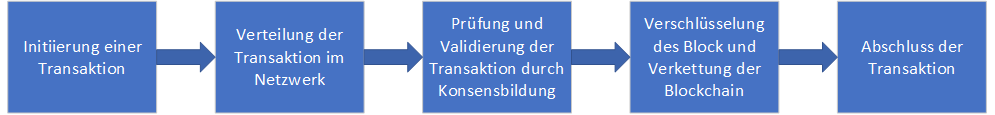
\includegraphics[width=\textwidth]{transaktions-ablauf.png}
	\caption{Vereinfachter Transaktionsablauf. Quelle: Fraunhofer FIT}
	\label{fig:transaktionsablauf}
\end{figure}

Zunächst wird die durchzuführende Transaktion im Netzwerk verteilt. Anschließend fassen die Netzwerkteilnehmer mehrere Transaktionen zu einem Block zusammen und versuchen durch eine Konsensbildung die Transaktionen zu validieren. Die Validierung findet bei der Blockchain-Technologie mit dem sogenannten Proof-Of-Work statt, welche es fordert das aus den Transaktionen und dem vorherigen Block ein Hash-Wert mit einer bestimmten Voraussetzung gebildet wird. Nachdem ein Netzwerkteilnehmer ein validen Hash-Wert ermittelt hat, werden der Block an die Kette angehangen und im Netzwerk verteilt. Alle anderen Teilnehmer überprüfen die Erweiterung der Kette. Falls die neue Blockchain nicht den Ansprüchen der Voraussetzung entspricht, wird die Erweiterung abgelehnt und die vorherige Kette zurückgegeben, andernfalls wird die erweiterte Blockchain übernommen. Anschließend ist die Transaktion erfolgreich durchgeführt.


\subsection{Blockaufbau}
\label{subsec:blockaufbau}
Ein Block besteht aus dem vorherigen Block-Hash-wert, den Transaktionen und dem neuen Hash-wert. Die Verkettung der Blöcke findet über den vorherigen Block-hashwert statt, indem der 

Hash eines Blockes besteht aus

-- Hash des vorherigen Blockes

-- Merkle-Root = Hash-Tree aus mehrere Transaktionen

-- Nonce = frei wählbarer Wert, um die Anforderung der Blockchain zu bewerkstelligen



-- Transaktionen

\subsection{Proof-Of-Work}
\label{subsec:proofofwork}
